\section{Описание реализации}

В данном разделе приводится краткое описание реализации решения на языке С++ с 
использованием возможностей инструментария Qt и его библиотеки для языка С++, а 
также с использованием инструментария, реализованного в рамках tabexchange.

\subsection{Внутреннее представление ограничения}

В качестве внутреннего представления отдельных ограничений используются 
специальные структуры: 

\begin{itemize}
 \item ExchangeRestrictDescription,
 \item ParamRestrictDescription,
\end{itemize}

наследующие тип RescrictDescription. Структуры содержат поля для хранения 
информации согласно описанию внутреннего представления (см. 
раздел~\ref{subsec:inner}) с дополнительным полем для идентификатора объекта - 
текстового идентификатора обмена (параметра). Это нужно для того, чтобы 
избавить фабрику обработчиков от необходимости взаимодействовать с полной 
иерархией объектов хранилища конфигурации анализатора.

Дополнительно в рамках этих структур реализованы методы для сохранения и 
загрузки полей из контейнера QSettings, а также метод для загрузки 
значений полей при импорте XML-описания протокола.

Структуры определены в файлах tabexchange/analyzercore.[h|cpp].

\subsection{Контейнеры для описания ограничений}

Для хранения внутреннего представления описания ограничений были реализованы 
контейнеры
\begin{itemize}
 \item ExchangeRestrictionContainer,
 \item ParamRestrictionContainer.
\end{itemize}

Контейнеры реализованы на базе класса NamedObjectContainer, используемого в 
tabexchange для создания контейнеров для именованных объектов с возможностью 
добавления, использования, редактирования (с оповещением классов-пользователей 
контейнера) элементов, а также автоматического сохранения содержимого 
контейнера в пользовательский репозиторий Анализатора MIL STD-1553B и 
последующей 
загрузки.

Именами в контейнерах служат текстовые идентификаторы: для обменов - 
идентификаторы сообщений, совпадающие с таковыми в контейнере описаний 
сообщений MessageContainer, для параметров - пара \textit{(имя\_сообщения, 
имя\_параметра)}, позволяющая также найти описание параметра в 
контейнере описания параметров ParameterContainer.

В качестве хранимых объектов используются массивы описаний ограничений, 
соответствующих каждому из типов обменов (параметров).

В рамках данной работы в класс TabExchangeImpl были добавлены методы для 
получения данных контейнеров.

Создание объектов контейнеров, а также реакция на запросы загрузки и сохранения 
данных в репозитории происходит в объекте класса TabExchangeImpl.

\subsection{Импорт описания ограничений}

Импорт файла описания протокола в tabexchange выполняется при помощи следующих 
классов:

\begin{itemize}
 \item BDPivImporter (файл tabexchange/mppexportimport.cpp) - класс, 
реализующий разбор XML-файла описания протокола преобразованием в представление 
QSettings, используемое в Qt-приложениях для хранения конфигурации в виде пар 
\textit{(ключ, значение)} с иерархией ключей. Объект класса заворачивается в 
функцию read(), передаваемую QSettings::registerFormat() для обобщённой 
обработки конфигурационных файлов различных форматов;.
 \item MPPExportImportModel, MPPExportImportDialog (файлы 
mppexportimport.cpp, mppexportimport.h в директории tabexchange) - классы, 
реализующие диалоговое окно импорта конфигурационного файла с возможностью 
разрешения конфликтов импорта.
\end{itemize}

В реализации анализатора ограничений были внесены следующие изменения:

\begin{itemize}
\item в класс BDPivImporter добавлена обработка XML-тегов <restrict> и 
<restricts>;
\item в метод MPPExportImportDialog::accept() добавлено заполнение контейнеров 
ExchangeRestrictionContainer и ParamRestrictionContainer в соответствии с 
описанием ограничений в загружаемом файле описания протокола.
\end{itemize}

\subsection{Контейнеры для сообщений и параметров}

В tabexchange реализованы специальные контейнеры для работы с описаниями 
сообщений и параметров:

\begin{itemize}
 \item MessageContainer,
 \item ParameterContainer.
\end{itemize}

В MessageContainer хранятся описания сообщений, в том числе шаблонные (одному 
описанию сообщения может соответствовать несколько реальных типов обменов). 
После незначительных изменений в коде контейнера, он используется в реализации 
анализатора ограничений для получения внутренних идентификаторов обменов (для 
каналов MIL STD-1553B, например, командных слов обмена). Внутренние 
идентификаторы обменов используются ядром анализатора для быстрого определения 
типа полученного обмена в обработчике события \textit{addExchange()}.

В ParameterContainer хранятся описания параметров, получаемых из сообщений, а 
также производится вычисление значений параметров при регистрации очередного 
обмена. В рамках данной работы в реализацию контейнера была добавлена рассылка 
уведомления о получении нового значения параметра (с использованием механизма 
``сигнал-слот'', реализованного в инструментарии Qt). Это уведомление 
используется ядром анализатора для запуска соответствующих обработчиков 
ограничений.

\subsection{Обработчики ограничений}

Для классов обработчиков ограничений описаны соответствующие базовые классы 
(файлы analyzercore.[cpp|h] в директории tabexchange):

\begin{itemize}
 \item AnalyzerExchangeCheckerBase,
 \item AnalyzerParamCheckerBase.
\end{itemize}

Эти классы содержат описание сигнала \textit{report()}, используемого для 
уведомления о новой строке отчёта, а также прототип чистой виртуальной функции 
\textit{check()}, принимающей в качестве аргументов:

\begin{itemize}
 \item для обменов - константный указатель на объект;
 \item для параметров - текстовый идентификатор параметра и константный 
указатель на структуру ParamValue, содержащую последнее полученное значение 
параметра и время его получения.
\end{itemize}

Все классы, реализующие обработку ограничений для обменов или параметров, 
должны наследоваться от одного из этих базовых классов.

Реализация обработчиков конкретных ограничений приводится в файлах 
analyzerfactory.[cpp|h] в директории tabexchange.

\subsection{Фабрики обработчиков ограничений}

Для создания и раздачи объектов обработчиков ограничений реализованы два класса 
фабрик объектов:

\begin{itemize}
 \item ExchangeCheckerFactory,
 \item ParamCheckerFactory,
\end{itemize}

реализующие фабрику обработчиков ограничений для обменов и параметров 
соответственно.

Реализация фабрик обработчиков содержит всю логику создания новых объектов 
обработчиков и выдачи уже существующих. В частности:

\begin{itemize}
 \item ExchangeCheckerFactory хранит множество пар 
\textit{(имя\_последовательности, обработчик)} для обработчиков ограничений на 
последовательность обменов. Для хранения множества используется тип данных 
QMap<QString, ExchangeSequenceChecker *>, реализующий ассоциативный массив на 
основе хэш-таблицы;
 \item ParamCheckerFactory хранит множество пар \textit{(имя\_группы, 
обработчик)} для обработчиков ограничений на группы связанных параметров. Для 
хранения множества используется тип данных QMap<QString, ParamBindChecker *>, 
реализующий ассоциативный массив на основе хэш-таблицы;
 \item ParamCheckerFactory хранит множество пар \textit{(ID\_параметра, 
обработчик)} для обработчиков ограничений на пороговые значения параметров. Это 
сделано для реализации механизма ``подавления'' ненужных сообщений внутри 
обработчика (если значение параметра пересекло несколько пороговых, сообщение 
будет выведено для порога с самым высоким уровнем критичности). Таким образом, 
для каждого параметра с наложенными ограничениями на пороговые значения будет 
создан только один обработчик, следящий за всеми порогами сразу. Для хранения 
множества используется тип данных QMap<QString, ParamThresholdChecker *>, 
реализующий ассоциативный массив на основе хэш-таблицы.
\end{itemize}

\subsection{Ядро анализатора}

Ядро анализатора ограничений представлено классом AnalyzerCore в файлах 
analyzercore.[cpp|h] директории tabexchange.

Объект класса AnalyzerCore содержит следующие (скрытые) поля данных:

\begin{itemize}
 \item \textit{mExchangeCheckers} - отображение множества внутренних 
идентификаторов обменов на списки обработчиков ограничений. Для хранения 
отображения используется тип данных QMap<ExchangeSignature, 
AnalyzerExchangeCheckers>, реализующий ассоциативный массив на основе 
хэш-таблицы;
 \item \textit{mParamCheckers} - отображение множества текстовых 
идентификаторов параметров на списки обработчиков ограничений. Для хранения 
отображения используется тип данных QMap<QString, AnalyzerParamCheckers> , 
реализующий ассоциативный массив на основе хэш-таблицы.
\end{itemize}

Класс AnalyzerCore предоставляет следующий набор методов для управления 
списками обработчиков ограничений:

\begin{itemize}
 \item \textit{addExchangeAnalyzer(signature, checker)} - добавляет 
обработчик ограничения для обменов с заданным внутренним идентификатором 
(signature);
 \item \textit{clearExchangeAnalyzers(signature)} - удаляет все обработчики 
ограничений для обменов с заданным внутренним идентификатором (signature);
 \item \textit{addParamAnalyzer(paramId, checker)} - добавляет обработчик 
ограничения для параметра с заданным текстовым идентификатором;
 \item \textit{clearParamAnalyzers(paramId)} - удаляет все обработчики 
ограничений для параметра с заданным текстовым идентификатором.
\end{itemize}

Для получения информации о новых обменах и значениях параметров используются 
слоты Qt:

\begin{itemize}
 \item \textit{onAddExchange(exch)} - реакция на регистрацию нового обмена 
\textit{exch} в системе;
 \item \textit{onParamValueUpdated(paramId, paramValue)} - реакция на 
обновление значения параметра с текстовым идентификатором \textit{paramId}.
\end{itemize}

Для перенаправления сообщений об ошибках от обработчиков к внешним потребителям 
реализован скрытый (private) слот \textit{onReport(item)}, перенаправляющий 
уведомление в сигнал \textit{report(item)}.

\subsection{Конфигуратор}

Для того, чтобы собрать процедуры подготовки ядра анализатора и установку всех 
связей в одном месте, реализован специальный вспомогательный класс 
AnalyzerConfigurator, определённый в файлах analyzerconfigurator.[cpp|h]. 

Объект класса выступает в качестве посредника между ядром анализатора 
и набором внешних контейнеров:

\begin{itemize}
 \item MessageContainer,
 \item ParameterContainer,
 \item ExchangeRestrictionContainer,
 \item ParamRestrictionContainer.
\end{itemize}

Задачи конфигуратора:

\begin{itemize}
 \item получение событий об обновлениях контейнеров с конфигурацией анализатора 
и вызов соответствующих методов ядра;
 \item конфигурация контейнера параметров для рассылки уведомлений об 
изменениях значений наблюдаемых параметров;
 \item преобразование текстовых идентификаторов сообщений во внутренние 
идентификаторы (с использованием инструментария MessageContainer).
\end{itemize}

\subsection{Строка отчёта анализатора}
\label{subsec:reportitem}

Каждая строка отчёта анализатора представляется объектом класса 
AnalyzerReportItem, описанного в файле analyzercore.h.

Строка отчёта анализатора содержит следующие поля данных:

\begin{itemize}
 \item время возникновения события;
 \item строка сообщения;
 \item уровень критичности ошибки;
 \item указатель на обмен, ``спровоцировавший'' возникновение ошибки.
\end{itemize}

Объекты этого класса рассылаются обработчиками ограничений при возникновении 
ошибок. Объект передаётся в ядро анализатора для пересылки, после чего 
отправляется модели вкладки отчёта анализатора для отображения ошибки в 
пользовательском интерфейсе Анализатора MIL STD-1553B.

\subsection{Вкладка анализатора}

Вкладка анализатора реализована классами

\begin{itemize}
 \item AnalyzerReportTab,
 \item AnalyzerReportModel
\end{itemize}

в файлах analyzerreporttab.[cpp|h] в директории tabexchange.

Вкладка анализатора представляет собой таблицу с колонками, соответствующими 
полям данных строки отчёта анализатора (см. раздел~\ref{subsec:reportitem}). 
Данные появляются в таблице автоматически по мере работы анализатора, что 
позволяет использовать анализатор в режиме регистрации обменов в реальном 
времени. Очистка отчёта происходит по запросу пользователя (при нажатии на 
кнопку ``Очистить'' в графическом интерфейсе пользователя Анализатора MIL 
STD-1553B).

Снимок экрана пользовательского интерфейса анализатора ограничений предложен на 
рисунке~\ref{fig:opermon_ui}.

\begin{figure}[ht]
 \centering
 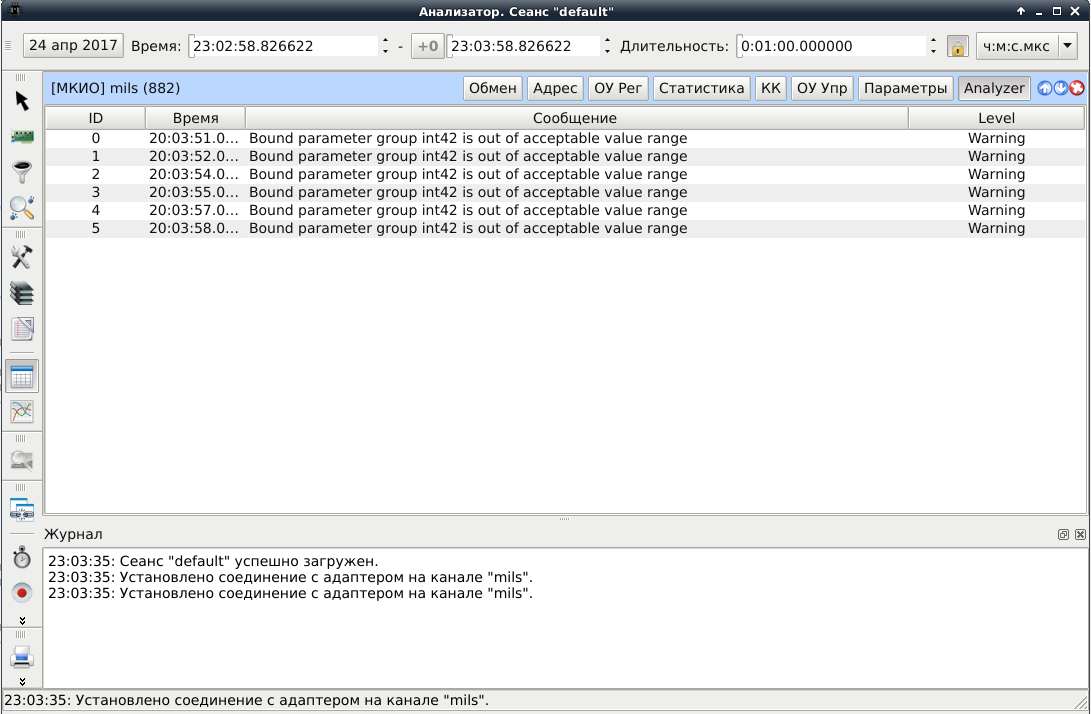
\includegraphics[scale=0.5]{opermon_ui}
 \caption{Пользовательский интерфейс анализатора ограничений}
 \label{fig:opermon_ui}
\end{figure}

Объект модели вкладки (класса AnalyzerReportModel) является получателем новых 
зарегистрированных обменов (принимая указатель на обмен в функции 
\textit{onAddExchange(exch)}), после чего перенаправляет событие в 
виде собственного сигнала \textit{addExchange(exch)}.

При создании объектов вкладки создаётся объект ядра анализатора и конфигуратор, 
а также проводится соединение сигналов и слотов для работы анализатора:

\begin{enumerate}
 \item сигнал \textit{paramValueUpdated} контейнера параметров привязывается к 
слоту \textit{onParamValueUpdated} ядра анализатора;
 \item сигнал \textit{addExchange} модели вкладки привязывается к слоту 
\textit{onAddExchange} ядра анализатора;
 \item сигнал \textit{report} ядра анализатора привязывается к слоту 
\textit{getReportItem} модели вкладки.
\end{enumerate}

Создание объектов вкладки происходит в фабрике каналов средства (файл 
sma/channelfactory\_su.cpp).